\documentclass[12pt]{article}
\usepackage{hyperref}
\usepackage[a4paper]{geometry}
\usepackage{graphicx}
\usepackage{listings}
\usepackage{multirow}

\newcommand{\fitxategi}[1] {\underline{\textit{#1}}}
\newcommand{\metodo}[1] {\textit{#1}}
\newcommand{\aldagai}[1] {\textit{#1}}
\newcommand{\tekla}[1] {\textbf{#1}}
\newcommand{\erref}[1] {\textbf{\ref{#1}}}

\renewcommand{\contentsname}{Edukiak}
\renewcommand{\refname}{Erreferentziak}
\renewcommand{\abstractname}{Laburpena}


\geometry{
 a4paper,
 total={170mm,257mm},
 left=2cm,
 top=2cm,
 }


\title{KbG proiektua: 3. eta 4. faseak}
\author{
        Oier Irazabal\\
        Jesus Calleja
}
\date{\today}



\begin{document}
\maketitle

%\begin{abstract}
%This is the paper's abstract \ldots
%\end{abstract}

\tableofcontents

\vspace{0.7cm}
\begin{center}
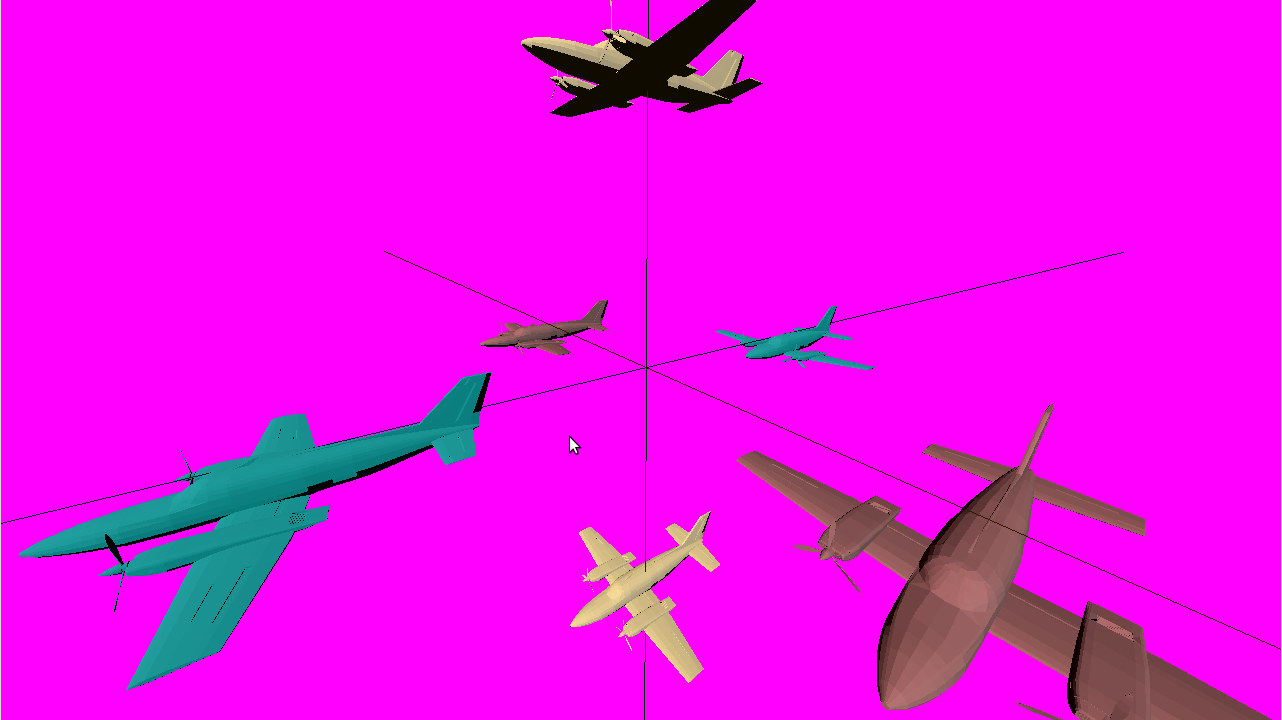
\includegraphics[scale=0.24]{fase_34_portada.png}\\
\end{center}

\pagebreak

\section{Kamera}

Fase honetan lortutako inplementazioa bi kamera motaren txertaketa izan da. Orain arte ingurunearen ikuspegi finko eta ez-fidela genuen. Proiekzioa ortografikoa zen; hau da, argi-izpiak Z ardatzarekiko paraleloak ziren, sakoneraren nozioa galduz. Gainera, kamera jatorrian geldi zegoen, objektuak izanik mugitu daitezken bakarrak.\\

Orain, bi kamera mota berri aukera daitezke: libreki mugi daitekeen perspektibazkoa, eta ibiltaria. \tekla{C} tekla sakatuz gero, kamera-motaz aldatzen da. Kamera hautatzeko gai izateaz gain, kamera transformatu ahal izateko, \tekla{K} tekla sakatzea dago, aukeratutako transformazioa kamerari aplikatzeko eta ez objektuari. Aitzitik, objektuak transformatzeko berriz, \tekla{O} tekla sakatu behar da.\\

Ideia teorikoak finkatu ditugu, baina nola lor daitezke orain arte aipatutako emaitza guztiak? Zerk osatzen du kamera bat?
Alde batetik, zein kamera motarekin ari garen hartu behar da kontutan, bestetik proiekzio motaz aldatu behar da hautatutako kameraren arabera, eta azkenik kameraren mugimendua eta biraketa simulatu behar dira. Horretarako hurrengo datu-egitura erabiliko dugu:

\begin{center}
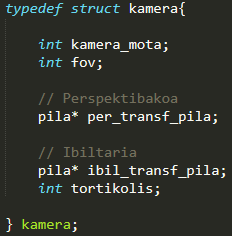
\includegraphics[scale=0.7]{kamera_struct.png}

\textbf{1. irudia}: kamera datu-egitura
\end{center}


Egiturako kideen azalpenak:

\begin{itemize}
\item \aldagai{kamera\_mota}: kamera ortografikoa, perspektibazkoa edo ibiltaria den adierazten du (ikus \erref{constants} atala)
\item \aldagai{fov}: Field Of View\cite{fov}, \erref{per_proj} atalean azaldua.
\item \aldagai{per\_transf\_pila}: perspektibazko kamera transformatzeko erabiltzen den aldaketa-pila, \erref{kam_sim} atalean azaldua.
\item \aldagai{ibil\_transf\_pila}: kamera ibiltaria transformatzeko erabiltzen den aldaketa-pila, \erref{kam_sim} atalean azaldua.
\item \aldagai{ibil\_gorabehera}: kamera ibiltariak plano horizontalarekiko daukan angeluarekiko proportzionala den balio bat. Bertikalki bira daitekeen eremua mugatzeko balio du.
\end{itemize}

\textbf{Oharra}: pila hauek objektuek erabiltzen duten bera dira.\\

Kamerarekin zerikusia duten metodo edo egitura guztiak \fitxategi{kamera.c} eta \fitxategi{kamera.h} fitxategietan daude.
Bestalde, \textbf{\_k} aldagaia \fitxategi{main.c} fitxategian definitzen eta hasieratzen da aldagai global bezala, kamera bakar bat erabiltzen duelako aplikazioak oraingoz.


\subsection{Perspektibazko proiekzioa}\label{per_proj}
Orain arte \fitxategi{display.c} fitxategiko \metodo{display()} metodoan, \metodo{glOrtho()} metodoa erabiltzen genuen proiekzio ortografikoa lortzeko. Hala ere, orain txertatutako beste bi kamera motek ez dute proiekzio bera erabiltzen, perspektibazkoa baizik. Beraz, proiekzio mota kamera motaren menpe geratuko da eta kamera ortografikoaz beste, \metodo{gluPerspective()}\cite{glu_perspective} izaneko metodoa erabiliko dugu proiekzio mota berria lortzeko.\\
Hona hemen pausu hau azaltzeko sasikodea:

\begin{center}
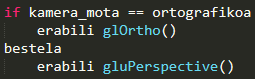
\includegraphics[scale=1]{kamera_projection.png}

\textbf{2. irudia}: Proiekzioa burutzeko sasikodea
\end{center}

Metodo berri honek lau argumentu hartzen ditu: \textit{FOV}, leihoaren aspektuaren erlazioa (aspect ratio)\cite{aspect_ratio} eta \textit{near} eta \textit{far} Z-planoak. Lau argumentuek \textit{frustum}\cite{frustum} izeneko bistaratze-eremua mugatuko dute. Irudi honek erakusten du \textit{frustum}-a nola mugatzen duten parametroek:

\begin{center}
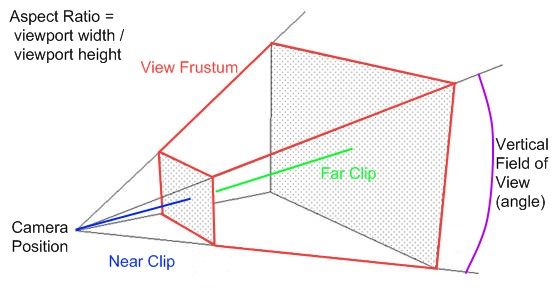
\includegraphics[scale=0.8]{kamera_frustum.jpg}

\textbf{3. irudia}: Kameraren \textit{frustum}-a
\end{center}

\textit{near} eta \textit{far} planoak kamerak sakoneran ikus dezakeen distantzia mugatzen dute. Aspektuaren erlazioak bistaratze-eremuaren proportzioa adierazten du, gure kasuan leihoaren bera izanik. Aldagai hau \fitxategi{display.c} fitxategiko \metodo{reshape()} metodoak kontrolatzen du, leihoaren dimentsioak aldatzea posible baita eta \aldagai{\_window\_ratio} aldagai globalean gordetzen da. Azkenik, \textit{FOV}ak kamerak zenbat ikus dezaken kontrolatzen du eta balioa kontrolatzeko kameraren egiturako \aldagai{fov} kidea erabiltzen da. \textit{FOV}a handiagoatuz, inguru handiago bat ikusi ahalko dugu, zoom efektua lortuz eta kamera ortografikoaren moduan \tekla{CTRL +} eta \tekla{CTRL -} teklen konbinaketekin kontrolatu ahal izango da.\\

\textit{near} eta \textit{far} planoaren balioak eta \textit{FOV}-aren hasierako balioa, minimoa eta maximoa \fitxategi{definitions.h} fitxategian definituta daude, lehenengo biak konstateak izanik (ikus \erref{constants} atala).


\subsection{Kameraren efektua}\label{kam_sim}

Transformazioak objektuei aplikatzen zaizkie. Kontraesana dirudien arren, izatez kameraren kontzeptua ez da existitzen ordenagailu bidezko grafikoetan. Kamera ezkerretara mugitzea simulatu nahi izanez gero, mundu guztia eskuinetarantz mugitu beharko da proportzio berean, ilusio hori lortzeko. Hau esanda, ondoriozta daiteke kamera simulatzeko objektu guztien transformazioa kargatu baino lehen kamerarena kargatu beharko dela.

\begin{center}
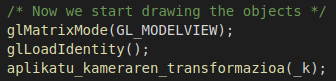
\includegraphics[scale=0.7]{kamera_transform.png}

\textbf{4. irudia}: kameraren transformazioaren aplikazioa
\end{center}

\textbf{Oharra}: Objektuak marrazteko begiztaren amaieran, identitate matrizea kargatu ostean, berriro aplikatu behar da kameraren transformazioa.\\

Kameraren transformazioa burutzeko \metodo{gluLookAt()}\cite{glu_lookat} metodoa erabiltzen dugu. Funtzio honek kameraren posizioa, begira dagoen puntuaren posizioa eta goranzko norabidea adierazten duen bektorea emanik, uneko matrizea (gure kasuan MODELVIEW) aldatzen du kameraren transformazioa simulatzeko. Datu hauek lortzeko, hasierako \aldagai{eye}, \aldagai{look} eta \aldagai{up} balioak (\metodo{gluLookAt()} funtzioaren parametroak hurrenez hurren) transformatko ditugu kameraren uneko posizioa eta errotazioa kalkulatzeko.

\begin{center}
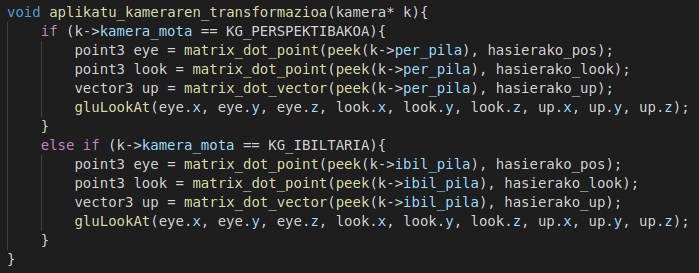
\includegraphics[scale=0.6]{kamera_lookat.png}

\textbf{5. irudia}: \metodo{gluLookAt()}-en erabilpena
\end{center}

\begin{center}
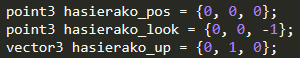
\includegraphics[scale=0.65]{kamera_hasierako_balioak.png}

\textbf{6. irudia}: hasierako balioak
\end{center}

Kalkuluak egiteko erabilitako bi biderketen metodoak \erref{matematikak}. atalean daude azalduta.


\subsection{Perspektibazko kamera}

Kamera hau libreki mugi eta bira daiteke espazioan, oso erabilgarria izanik ingurunea ikuspuntu askotatik aztertu ahal izateko. Adibidez, Blender\cite{blender} eta itxura horretako aplikazioek aukera hau eskaintzen dute.

\subsubsection{Transformazioak}

Kamerak translatzeko eta biratzeko aukera du, eskalatzea eta zizailatzeak zentzurik ez baitaukate. Bi aldaketa hauek lokalean zein globalean egin daitezke. Mugimendua globala denean, munduko X, Y eta Z ardatzetan emango da translazioa, lokalean aldiz, uneko begiradaren norabidearen araberakoa izango da. Biraketa globala denean, kamerak jatorriaren inguruan biratuko du hautatutako ardatzean, lokalean aldiz, kamera geldi geratuko da, begiradaren norabidea aldatuz.

\subsection{Kamera ibiltaria}

Pertsona baten mugimendua simulatzen duen kamera da. Perspektibazko kamerarekin alderatuta askatasun gutxiago dauka, alde batetik kamera $Y=0$ planoan zehar mugi daitekelako bakarrik eta mugitzeko eta biraketzeko aukera gutxiago dituelako. Gora eta behera geziekin aurrera eta atzera mugitzen da, ezker-eskuin geziekin alboetara biratzen du begirada eta \tekla{REPAG}-\tekla{AVPAG} teklekin gora eta beherantz biratzen du begirada. Azken biraketa hau mugatuta dago, ez baitauka zentzurik pertsona batek burua bertikalki edozein angelurekin biratu ahal izateak.


\subsubsection{Transformazioak}

Transformazio hauek kalkulu konplexuago bat eskatzen dute, ez baita bakarrik matrizeak aurretik edo atzetik biderkatzea bezain sinplea.\\
Arazoetariko bat kamera $Y=0$ planoan mantentzea da. Biraketa horizontalak ez dio honi trabarik egiten, baina bai bertikalak, lurrarekiko angelua aldatzen duenez, kameraren "aurrera" bektorea  biratzen duelako berarekin, $Y=0$ planoaren paralelo izateari utziz. Horretarako, kalkula dezakegu kamerak zein posiziotan bukatuko duen transformazioa burutzean, gero posizioaren altuerarekin translazio global bat aplikatzeko kontrako norabidean.

\begin{center}
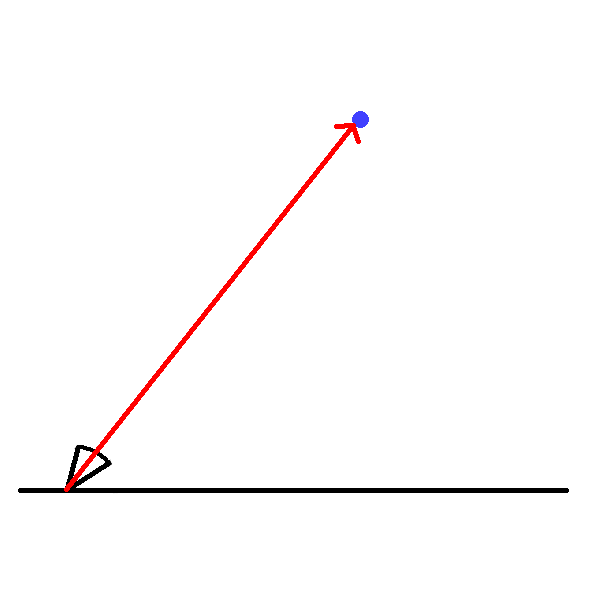
\includegraphics[scale=0.3]{kam_ibil_a1.png}
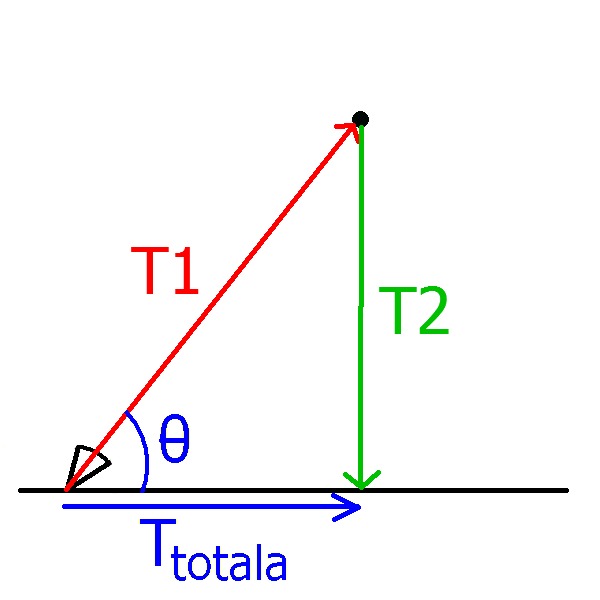
\includegraphics[scale=0.3]{kam_ibil_a1_sol.png}

\textbf{7. irudia}: Kamera ibiltariaren lehenengo arazoa
\end{center}

Hala ere, konponketa honek albo-ondorio bat dakar. Goiko eskuineko irudian ikus daitekenez, plano horizontalean aurreratutako distantzia ez da 1ekoa, bektorearen plano horizontalarekiko duen proiekzioaren luzera baino, $\cos(\theta)$ = $\cos$(KG\_THETA $\cdot$ k-$>$ibil\_gorabehera) zuzenki. Beraz, zenbat eta angelu bertikal handiagoa, hainbat eta pausu txikiagoa aurreratuko dugu, efektu errealistagoa emanez kamera ibiltariari eta albo-ondorioaz aprobetxatuz.\\

Bigarren arazoa lehenengoarekin lotuta dago. Kamera bertikalean biratu ondoren, horizontalean biratuz gero, kameraren posizioa geldi geratzen den arren, begirada ez da horizontalean biratzen, azpiko ezkerreko aldeko irudian ageri den moduan. Arazoa konpontzeko kameraren biraketa bertikala desegin behar da lehen, gero biratu horizontalean eta azkenik berregin biraketa bertikala, desio den transformazioa lortzeko. Konponketa honek ez dauka albo-ondoriorik.

\begin{center}
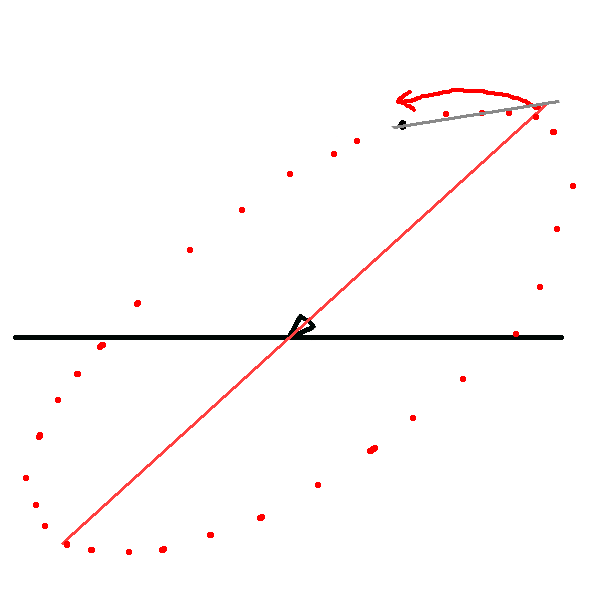
\includegraphics[scale=0.3]{kam_ibil_b1.png}
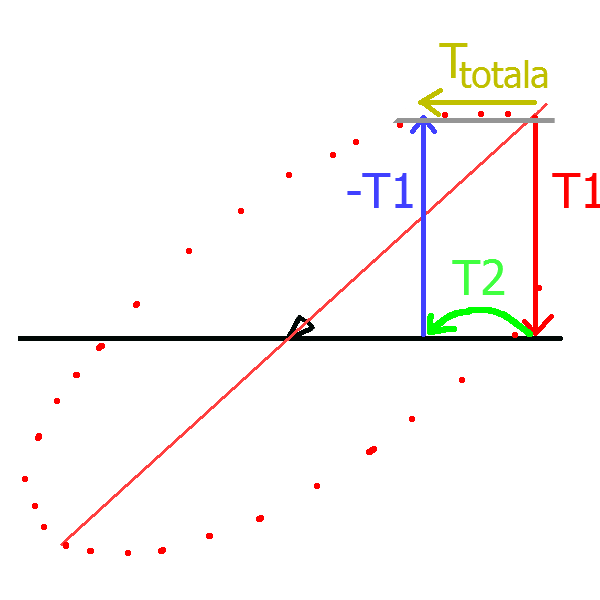
\includegraphics[scale=0.3]{kam_ibil_b1_sol.png}

\textbf{8. irudia}: Kamera ibiltariaren bigarren arazoa
\end{center}

Matrizeen konbinaketa hau ezinbestekoa da kamera ibiltariaren aldaketa-pilak ondo funtziona dezan, bai aldaketak desegiteko eta bai berregiteko, konbinazioan parte hartzen duten matrize guztiak "pack" berean aplika daitezen.


\subsection{Aldaketak desegitea eta berregitea}\label{aldaketak}

Objektuekin bezala, kamerari aplikatutako transformazioak desegitea eta berregitea badago, pila mota berdinak baitira. Kamera mota bakoitza bata-bestearekiko independentea izatea nahi dugunez, perspektibazko kamerarentzako pila bat eta ibiltariarentzako beste bat sortuko ditugu (ikus \textbf{1. irudia}). Demagun perspektibazko kamerari edozein hiru transformazio lokal aplikatzen dioguzela, orduan pilaren egoera hurrengoa izango zen:\\
transformazioen ordena lehenik \textbf{M1}, gero \textbf{M2} eta azkenik \textbf{M3} izanik eta \textbf{I} identitate matrizea,

\begin{center}
\begin{tabular}{r|r|r}
 \cline{2-2}
 $top \rightarrow$ & $\textbf{M3} \cdot \textbf{M2} \cdot \textbf{M1}$ & \\
 \cline{2-2}
 & $\textbf{M2} \cdot \textbf{M1}$ & \\
 \cline{2-2}
 & $\textbf{M1}$ & \hspace{0.5cm} ($\textbf{M1} \cdot \textbf{I} = \textbf{M1}$) \\
 \cline{2-2}
 & $\textbf{I}$ & \\
 \cline{2-2}
\end{tabular}

\textbf{1. diagrama}: Pilaren erabilpena.
\end{center}

Pilaren erabilera lau ekintzetan banatzen da:

\begin{itemize}
\item \textbf{Pila sortzea}. Identitate matrizea gordetzen duen pila bat itzultzen du \metodo{pila\_sortu()} metodoa erabiliz.

\item \textbf{Pilaratzea}. Matrize berri bat pilaratzen du. Orokorrean matrize hau aurreko matrizearen transformazio bat izango da, \metodo{peek()} (pilaren gaineko matrizea lortzeko) eta \metodo{push} (matrizea pilaratzeko) konbinatuz.

\item \textbf{Aldaketak desegitea}. Metodo honek azkenengo matrizea apuntatzen duen \textit{pointer}-a\cite{pointer} aurreko matrizera mugitzen du azkenengo posizioko elementua ezabatu gabe, azken aurreko aldaketa erakutsiz. Ekintza hau \metodo{pop()} metodoak burutzen du.

\item \textbf{Aldaketak berregitea}. Aurreko ekintzaren kontrakoa da, \textit{pointer}-a elementu bat aurrerago eramanez, \metodo{depop()} metodoak burutzen duena. 
\end{itemize}

Funtsean, pila bi zentzutara lotutako lista estekatu bat da. Datu egitura honek bi propietate garrantzitsu ematen dizkigu: pila nahi beste hazi ahal izatea (memoriarik gabe geratu arte) eta bi noranzko nabigagarritasuna, pilaren azken elementuari apuntatzen dion \textit{pointer}-a bi aldeetara mugitzea ahalbidetzen duena (\metodo{pop()} eta \metodo{depop()}).\\
Hona hemen datu-egituraren diagrama bat:

\begin{center}

\fbox{\textbf{I}} $\leftrightarrow$ \fbox{\textbf{M1}} $\leftrightarrow$ \fbox{\textbf{M2} $\cdot$ \textbf{M1}} $\leftrightarrow$ \fbox{\textbf{M3} $\cdot$ \textbf{M2} $\cdot$ \textbf{M1}}

\hspace{5.5cm} $\uparrow$

\hspace{5.5cm} top

\textbf{2. diagrama}: Pilaren elementuen arteko lotura.
\end{center}




\section{Argia}

\subsection{Z-buffer}

Orain arte objektuen \textit{wireframe}\cite{wireframe} bat marraztu dugu, orain berriz, gainazalak marraztu behar ditugula, beharrezkoa da jakitea zein aurpegi dagoen bata bestearen atzean. Horretarako, Z-bufferra gaitu behar da \fitxategi{main.c-ko} \metodo{init()} funtzioan, kameratik hurbilen dauden pixelak bakarrik marrazteko.

\begin{lstlisting}[language=C]
glutInitDisplayMode(GLUT_SINGLE | GLUT_RGB | GLUT_DEPTH );
glEnable(GL_DEPTH_TEST );
\end{lstlisting}

Kontuan hartu behar da buffer berria gaitu dugunez, bufferra garbitu behar da errenderizazio iterazio bakoitzeko.

\begin{lstlisting}[language=C]
glClear(GL_COLOR_BUFFER_BIT | GL_DEPTH_BUFFER_BIT );
\end{lstlisting}

\subsection{Aurpegien bektore normalak}

Errealitatean bezala, argi-izpiek ez dute berdin argiztatzen plano desberdinetan dauden gainazalak, gainazalaren eta argi-izpien arteko angeluaren menpe egonik. Gure programan angelu bera kalkulatu beharko dugu eta horretarako, lehenik objektuen aurpegien bektore normalak (edo perpendikularrak) kalkulatu beharko ditugu. Balioak gordetzeko \fitxategi{definitions.h}-ko \aldagai{face} egituran \aldagai{vector3 normal\_vector} atributua gehitu dugu.\\

Normalak kalkulatzeko, objektua kargatzerakoan aurpegi bakoitzaren lehen hiru erpinak hartzen ditugu. Kalkulu hau bakarrik behin burutu behar da, transformazioek normalei ere eragiten baitie. Kalkulua burutzeko \fitxategi{matematikak.c} fitxategiko \metodo{cross\_product()} funtzioaz baliatuko gara.\\

Azkenik, OpenGL-k normalak erabili ditzan, \fitxategi{display.c} fitxategiko \metodo{display()} funtzioan, erpinen posizioa eman baino lehen, erpin horrek osatzen duen aurpegiaren bektore normala kargatuko dugu. Hori egiteko \metodo{glNormal3d()} funtzioa erabiliko dugu bektore normalaren x, y eta z koordenatuak pasatuz.\\

\textbf{Oharra}: Erpin bakoitza aurpegi bat baino gehiagoren parte izan daitekenez, prozesatzen den azken aurpegiaren normalaren balioa hartuko du, aurreko balioaren gainean idatziko baita normal berriaren balioa.
 
\subsection{Erazagupena}

Bizitza errealeko argiak simulatzen dituzten hiru argi mota inplementatu ditugu: eguzkia, bonbila eta fokua.\\

Eguzkia direkzionala da, edozein puntutan bere argiak angelu berarekin inziditzen baitu. Beraz, bakarrik hartu behar dugu kontutan norabidea (eguzkia infinituan baitago). Beste biak posizionalak dira, argi-izpiak posizio batetik era erradial eta dibergente batean abiatuz. Hala ere, bonbilaren kasuan, norabideak ez du garrantziarik, norabide guztietan igortzen baitu argia. Posizoa eta norabidea, biak kontutan hartzen dituen argi mota bakarra fokua da.

\begin{center}
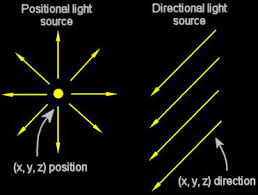
\includegraphics[scale=0.7]{argia_posdirek.jpeg}

\textbf{9. irudia}: argi posizionala eta direkzionala.
\end{center}

\aldagai{OpenGLk} desberdintasn hau nabaritzen du \aldagai{GL\_POSITION-i} pasatzen diogunaren arabera: bektorearen azken elementua 0 bada, bektore bat bezala ulertuko du; beraz, \aldagai{OpenGLk} eguzki-motatzat hartuko du argi hori. Pasatzen diogun bektorearen azken balioa 1 bada, argi posizional bezala tratatuko du.\\

\begin{center}
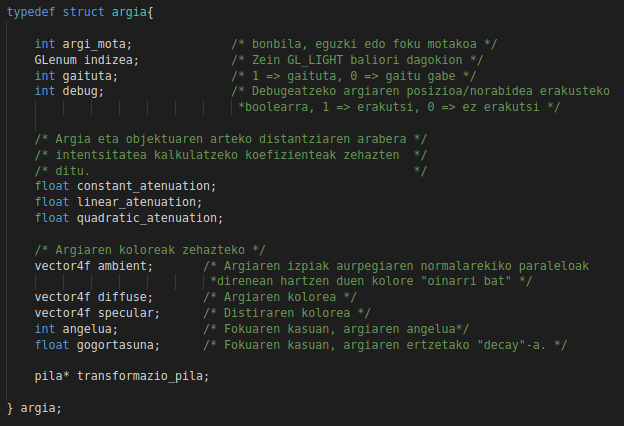
\includegraphics[scale=2.5]{argia_estruktura.png}

\textbf{10. irudia}: argia estruktura.
\end{center}

Goiko irudian agertzen den esstrukturaz baliatuz, argairen datuak gordeko ditugu. \aldagai{argi\_mota} eguzki -0- , bonbila -1- edo foku -2- artean desberdintzeko balio du. \aldagai{indizea} zehazten du zein argiri dagokion instantzia horien datuak. \aldagai{gaituta} adierazten du ea argia piztuta dagoenentz. \aldagai{angelua} fokuaren kasuan honek daukan zabalera zehazteko balio du. \aldagai{diffuse} aldagaiak argiaren kolorea zehazten du. \aldagai{ambient} hitzak esaten duen moduan, argiaren ingurumenaren kolorea zehazten du. \aldagai{specular} objektua distiratsua bada, honen kolorea kalkulatzeko zehazten den argiaren kolore-mota hau balio du. \aldagai{gogortasuna} argitik iluntasunera dagoen espektroaren "gogortasuna"zehazten du. Amaitzeko, \aldagai{transformazio\_pila} argiari egindako transfromazio matrizeen pila gordetzeko balio du.\\

Orain arte, \aldagai{double} motako zenbakiekin lan egin dugu, baina argiak definitzeko glLightfv-ko parametroak \aldagai{float} motakoak direnez, \aldagai{vector4f} estruktura sortu dugu \fitxategi{definitions.h-n}. Estruktura honek lau \aldagai{float-eko} bektorea gordetzen du.\\


\subsection{Inplementazioa}

Zortzi argi definitu ditugu hasieran (3 extra), defektuz desgaituta.\\
Argiztapena gaitzeko \tekla{ENTER} sakatu behar da, \metodo{glEnable(GL\_LIGHTING)} metodoa deituko duena. Ostean, argi bakoitza pizteko, \tekla{F1} - \tekla{F8} teklak sakatuz, \metodo{argiaren\_egoera\_aldatu()} metodoa deituko duena, dagokion argia piztuz edo itzaliz. Argia gaituta bazegoen, desgaitu egiten du \metodo{glDisable()} funtzioari argiaren indizea pasatuz, kontrako kasuan \metodo{glEnable()} erabiliz.\\

Argiek objektuetan eragin dezaten, objektuak marraztu baino lehen \metodo{argia\_kargatu()} metodoa erabili behar da argi bakoitzarekin, desgaituta egon arren. Metodo honek argi mota bakoitzaren arabera, argiaren posizioa, norabidea, fokuaren zabalera... ezarriko ditu.\\

Batzuetan argiaren posizioa edo norabideaz ahaztea gerta daitekenez, \textit{debug} tekla bat inplementatu dugu, argiaren datuak marraztuko dituena. Ezinbestekoa da aurretik \tekla{A} sakatzea eta gaitutako argi bat aukeratuta izatea. Argiaren motaren arabera, datu ezberdinak emango dira:

\begin{itemize}

\item Eguzkiaren kasuan, jatorrian zentratutako lerro batek adieraziko du izpien norabidea.

\item Bonbilaren kasuan, posizioa adieraziko dute hiru lerroren ebaketak (ardatz bakoitzeko bat, munduaren jatorriaren ardatzen bezala).

\item Fokuaren kasuan, bonbilaren bezala adieraziko da posizioa eta norabidea posizioan zentratutako lerro luzeago batek adieraziko du.

\end{itemize}

\textbf{Oharra}: hasieran, bai posizioak eta norabideak munduko jatorria adierazten duten ardatzekin bat egingo dute eta baliteke ezin ikusi ahal izatea.\\

Hona hemen adibide bat:
\begin{center}
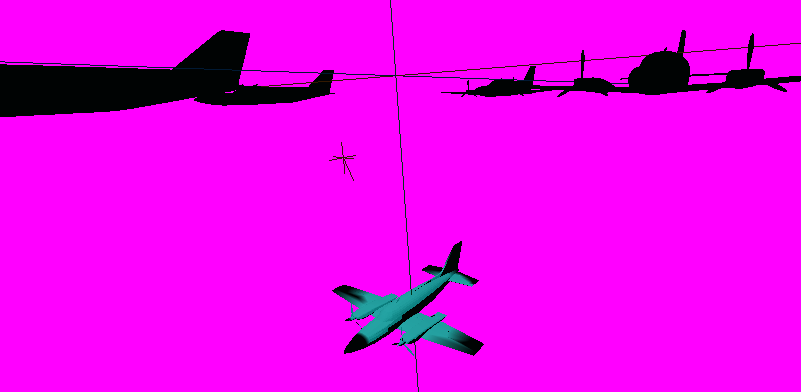
\includegraphics[scale=2.2]{debug.png}

\textbf{11. irudia}: \textit{debug} laguntza.
\end{center}

Baina, nola pasatzen dizkiogu OpenGL-ri argiaren egiturako datuak?\\
Bi modu daude, elementu bakarreko datuak pasatzeko \metodo{glLightf(argiaren indizea, propietatea, datua)} metodoa erabiliko dugu, non 
propietatea fokuaren angelua \textit{(GL\_SPOT\_CUTOFF)}, atenuazio-faktore lineala \textit{GL\_CONSTANT\_ATTENUATION}... izan daitezken eta datua, berari dagokion kameraren egiturako datua; kasu honetan \aldagai{angelua} eta \aldagai{constant\_attenuation}, hurrenez hurren.\\

Elementu anitzeko balioak pasatzeko hurrengo metodoa erabiliko dugu:
\begin{lstlisting}[language=C]
glLightfv(argiaren indizea, propietatea, (float*) &datua);
\end{lstlisting}
Kasu honetan \textit{type punning}\cite{punning} bat erabiltzen dugu, datuak \aldagai{vector4f} egituran gordetzen baititugu eta funtzioak \aldagai{float} motako zerrenda batean eskatzen baitizkigu balioak. Praktika hau arriskutsua izan daiteken arren, bi datu-motek era berean errepresentatzen dituztenez memorian balioak, gure kasuan funtzionatzen du.

\subsection{Argien transformazioak}

Argi bakoitza transformatzeko, \tekla{1}etik \tekla{8}erako teklekin aukeratu behar da lehenik. Kameraren bezala, argiak bakarrik biratu eta mugitu daitezke. Hala ere, zenbait argi mota bakoitzak bere mugak ditu:

\begin{itemize}
\item Eguzki-argia bakarrik bira daiteke. Eguzkiaren definizioan esan bezala, kokapena ez delako erabiltzen kalkuluan, norabidea baizik.

\item Bonbila-argia bakarrik mugi daiteke. Inguru osoa argiztatzen duenez, ez dauka zentzurik biratzeak.

\item Fokuaren norabidearen biraketa posizioaren inguruan izango da, ez jatorriaren inguruan. Horretarako hiru transformazio konbinatu behar dira. Lenehik, posizioa desegin, gero biraketa eta azkenik posizioa berregin.

\end{itemize}

Transformazio guztiak era globalean emango dira. Beraz, ez dago hautatutako erreferentzia-sistema kontutan hartu beharrik.\\

\textbf{Oharra}: Argi motaz aldatzean, transformazioa hasieratzen da aldaketa guztiak galduz. Ez dauka zentzurik fokuaren posizioa gordetzeak eguzkiarentzako, esaterako.

\subsection{Fokuen angelua handitu edo txikitu}

Foku motako argia hautatuta badugu, argiztapen-eremua handitzean edo txikia daukagu. \tekla{+} edo \tekla{-} teklak sakatuz gero, fokuaren angelua aldatzen dugu, beti ere angelua 10 gradu eta 90 graduren artean egonik.

\section{Materialak}

Argiez gain, objektu bakoitzak bere materiala izatea ahalbidetu dugu OpenGLko materialak erabiliz.\\

Materiala estruktura sortu dugu \fitxategi{definitions.h} fitxategian eta \fitxategi{materiala.c}-n definitu ditugu materialekin erlazionatutako funtzioak.\\

SARTU MATERIALAN STRUCTEN KAPTURIE

Lehenengo hiru propietateek (\aldagai{ambient}, \aldagai{diffuse} eta \aldagai{specular}) materialek argiarekiko duten portaera definitzen dute. Laugarren propietateak (\aldagai{shininess}) materialaren distiraren kolorea definitzen du. Azken propietateak (\aldagai{emission}) materialak igortzen duen argiaren kolorea definitzen du.\\

Objektua kargatzerakoan defektuzko material bat ematen zaio, \url{http://devernay.free.fr/cours/opengl/materials.html} web-orritik ateratako \textit{cyan rubber}.

\subsection{Materialal fitxategitik irakurtzea}

Materialen fitxategi batetik kargatzeko, \fitxategi{materiala.c} fitxategian \metodo{read\_materiala()} sortu dugu eta hautatutako objektuaren materialari balioak esleitzen dizkio.\\

Materiala kargatzeko fitxategiak hurrengo formatua izango du, lerroz lerro:
\begin{enumerate}

\item Materialaren izena traola baten ostean. Adibidez: \#ruby.

\item \aldagai{ambient}

\item \aldagai{diffuse}

\item \aldagai{specular}

\item \aldagai{emission}

\item \aldagai{shininess}

\end{enumerate}

2-5 zenbakidun datuak 4 elementuko bektoreak dira eta euren elementuen banaketa zuriune batekin markatu beharko da.\\

Adibide bezala, \fitxategi{mat} direktorioan daude pare bat material adierazten duten testu-fitxategi.


\section{matematikak.c}\label{matematikak}

Kalkulu matematikoak fitxategi bat baino gehiagotik burutzen zirenez eta metodo berak behar zirenez, gure programak behar dituen kalkulu matematiko gutziak \fitxategi{matematikak.c} fitxategian gorde ditugu. Gehien bat matrizeak kudeatzen dituen arren, badauka eskalarrekin eta bektoreekin operatzen dituzten funtzioak.\\

Fitxategi honen abantailarik handiena transformazio-matrizeak sortzeko eta biderkatzeko ahalmena da. Horrela, fitxategi hau erabiltzen duten beste fitxategietan kode txukunagoa dute eta gainera, inplementazioa aldatu nahi badugu, bakarrik metodo bat aldatzea izango da, dena zentralizatuta baitago orain.

\pagebreak

\section{Konstante berriak}\label{constants}

Kameraren funtzionamendurako sartutako konstanteak hurrengoak dira:

\begin{itemize}
\item Kamera mota:
\begin{itemize}
\item KG\_ORTOGRAFIKOA
\item KG\_PERSPEKTIBAZKOA
\item KG\_IBILTARIA
\end{itemize}

\item Transformazioak zeini aplikatuko:
\begin{itemize}
\item KG\_TRANSFORMATU\_OBJEKTUA
\item KG\_TRANSFORMATU\_KAMERA
\item KG\_TRANSFORMATU\_ARGIA
\end{itemize}

\item Kameraren proiekzioaren balioak:
\begin{itemize}
\item KG\_ZNEAR
\item KG\_ZFAR
\item KG\_FOV\_INIT
\item KG\_FOV\_MIN
\item KG\_FOV\_MAX
\end{itemize}

\item (\fitxategi{kamera.c} fitxategian) Kamera ibiltariaren biraketa bertikalaren \textit{step} maximoa:
\begin{itemize}
\item IBIL\_MAX\_GORA\_BEHERA
\end{itemize}

\item Argi mota:
\begin{itemize}
\item KG\_EGUZKIA
\item KG\_BONBILA
\item KG\_FOKUA
\end{itemize}

\item (\fitxategi{io.c} fitxategian) Tekla berrien kodeak:
\begin{itemize}
\item F1 - F8 teklak. Argiak gaitzeko/desgaitzeko.
\item F11 tekla. Objektuaren materiala kargatzeko.
\end{itemize}

\end{itemize}

\pagebreak

\bibliographystyle{abbrv}
\bibliography{main}

\begin{thebibliography}{9}

\bibitem{fov} 
\underline{Field Of View}:\\
\url{https://en.wikipedia.org/wiki/Field_of_view}

\bibitem{glu_perspective} 
\underline{gluPerspective()}:\\
\url{https://www.khronos.org/registry/OpenGL-Refpages/gl2.1/xhtml/gluPerspective.xml}

\bibitem{aspect_ratio} 
\underline{Aspect Ratio}:\\
\url{https://en.wikipedia.org/wiki/Aspect_ratio_(image)}

\bibitem{frustum} 
\underline{Frustum}:\\
\url{https://en.wikipedia.org/wiki/Viewing_frustum}

\bibitem{glu_lookat} 
\underline{gluLookAt()}:\\
\url{https://www.khronos.org/registry/OpenGL-Refpages/gl2.1/xhtml/gluLookAt.xml}

\bibitem{blender} 
\underline{Blender}:\\
\url{https://www.blender.org/}

\bibitem{pointer} 
\underline{Pointer}:\\
\url{https://www.programiz.com/c-programming/c-pointers}

\bibitem{punning}
\underline{Type Punning}:\\
\url{https://en.wikipedia.org/wiki/Type_punning}

\bibitem{wireframe}
\underline{Wireframe}:\\
\url{https://pages.mtu.edu/~shene/COURSES/cs3621/NOTES/model/wireframe.html}



\end{thebibliography}


\end{document}
